\section{结果与分析}
\subsection{统一分组评价下的模型比较}
表\ref{tab:v2comparison}给出12种方法的完整比较。两条提出路线中，SOLAR-H的母体等权MAE较低，为0.7164；最强基线为ExtraTrees，对应0.7469。二者的母体配对误差差为-0.0305，95\% bootstrap区间为[-0.0693, 0.0086]，128个母体中有67个误差下降。误差差的区间跨零，且改善分布于约半数母体，表明平均收益伴随较大的药物间差异（图\ref{fig:v2comparison}）。

\begin{table}[htbp]\centering\small
\caption{主要嵌套评价与固定划分评价。主要指标先按种子计算再平均；固定划分列来自完整开发集训练后的397条固定记录。所有误差均使用log10尺度。}\label{tab:v2comparison}
\begin{tabular}{lrrrrr}\toprule
模型 & 母体MAE$\downarrow$ & MAE$\downarrow$ & RMSE$\downarrow$ & $R^2\uparrow$ & 固定母体MAE$\downarrow$\\\midrule
SOLAR-H & 0.716 & 0.752 & 1.002 & 0.388 & 0.759\\
ExtraTrees & 0.747 & 0.749 & 0.973 & 0.423 & 0.734\\
随机森林 & 0.759 & 0.770 & 0.993 & 0.400 & 0.791\\
TabM & 0.778 & 0.770 & 1.000 & 0.391 & 0.725\\
HGB & 0.789 & 0.744 & 0.953 & 0.446 & 0.810\\
RealMLP & 0.804 & 0.815 & 1.068 & 0.304 & 0.783\\
SOLAR-H$_0$ & 0.824 & 0.822 & 1.155 & 0.186 & 0.749\\
温度差分MLP & 0.837 & 0.795 & 1.051 & 0.327 & 0.844\\
普通MLP & 0.838 & 0.799 & 1.048 & 0.330 & 0.842\\
SOLAR-N & 0.888 & 0.848 & 1.284 & -0.012 & 0.756\\
Ridge & 0.895 & 0.956 & 1.235 & 0.070 & 0.985\\
均值预测 & 0.964 & 1.059 & 1.311 & -0.048 & 1.028\\
\bottomrule\end{tabular}\end{table}
表\ref{tab:v2comparison}中的排序差异反映了模型优化对象的不同。HGB取得较低的逐行MAE和RMSE，说明其迭代拟合残差的方式适合减少当前记录分布中的总体偏差；SOLAR-H在母体等权MAE上更优，则与其均衡训练目标一致。高频药物在逐行指标中具有较大影响，而SOLAR-H通过重加权提高低频母体的训练贡献，因此其主要价值体现在药物层面的平均表现。

Ridge仅表达描述符的加性线性关系，难以充分刻画结构性质与溶剂条件的非线性组合；随机森林、ExtraTrees和HGB的较低误差支持非线性分区的建模价值。SOLAR-H进一步将结构预测与温度响应分离，使结构树集成能够先学习主要的分子差异，再由验证风险决定条件分支的强度。固定配置消融中，关闭母体均衡使母体MAE升高，将温度增益设为1也明显增加误差，这两项对照分别检验均衡权重和响应收缩的作用，具体结果见表\ref{tab:v2ablation}。

TabM的参数共享集成和RealMLP的优化配置为描述符任务提供了较强的神经网络基线，但SOLAR-N未从双编码器与温度差分中获得相同收益。其误差分布出现较长右尾，最差母体MAE达到10.567，表明少数药物上的响应偏差对总体表现影响较大。由于SOLAR-N的预测含有$\tau r(z)$，结构斜率估计误差会随温度偏离参考值而放大；关闭温度分支后的改善与这一机制一致。SOLAR-H允许验证过程将温度增益降至零，从而提供了一条抑制此类误差传播的路径。

固定划分下，TabM的母体等权MAE最低，SOLAR-H的误差也高于ExtraTrees（表\ref{tab:v2comparison}）。排序随评价母体变化，说明模型对药物组成具有不同敏感性，也体现了多折分组评价对平均推广表现的检验价值。SOLAR-H平均拟合时间为0.698秒，ExtraTrees为0.106秒；增加响应估计和交互表示后，混合路线在当前规模下保持亚秒级拟合。
\begin{figure}[htbp]\centering
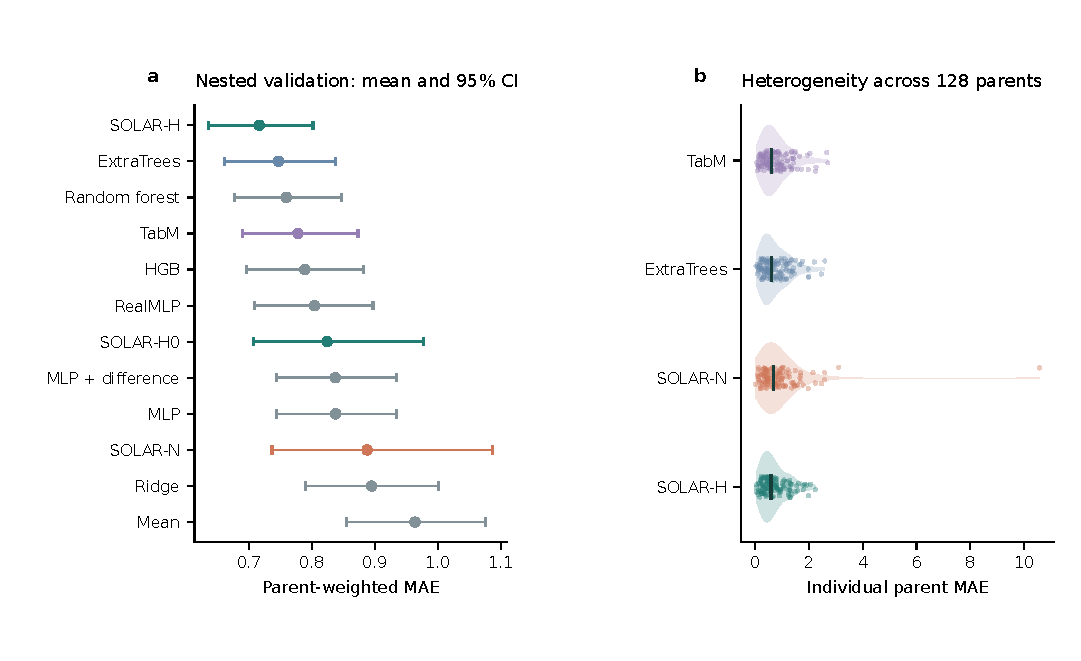
\includegraphics[width=\linewidth]{revision_v2/v2_comparison.pdf}
\caption{统一评价下的模型表现。\textbf{a} 128个母体的等权误差及2000次母体bootstrap的95\%区间。\textbf{b} 代表方法的母体误差分布，小点对应母体，短线表示中位数，密度形状描述分布。每个母体先平均三个种子的绝对误差。均值比较与母体分布共同呈现整体表现和误差集中程度。}
\label{fig:v2comparison}\end{figure}
\subsection{消融实验与数据规模}
如表\ref{tab:v2ablation}和图\ref{fig:v2ablation}所示，组件变体用于比较均衡权重、交互项及温度收缩的作用。
\begin{table}[htbp]\centering\small
\setlength{\tabcolsep}{5pt}
\caption{组件勾选消融结果。B为母体均衡，I为分子交互，T为温度分支，D为差分监督；$\checkmark$表示启用，--表示停用或不适用。$\gamma_{\rm CV}$表示沿用该外层折选定的增益，温度分支停用时增益记为0。误差差值以同路线完整模型为参照。}\label{tab:v2ablation}
\begin{tabular}{lcccccrr}\toprule
模型 & B & I & T & D & $\gamma$ & 母体MAE$\downarrow$ & $\Delta$MAE$\downarrow$\\\midrule
SOLAR-H$_0$ & $\checkmark$ & $\checkmark$ & $\checkmark$ & -- & $1$ & 0.8242 & +0.0000\\
SOLAR-H$_0$ & -- & $\checkmark$ & $\checkmark$ & -- & $1$ & 0.8407 & +0.0166\\
SOLAR-H$_0$ & $\checkmark$ & -- & $\checkmark$ & -- & $1$ & 0.7581 & -0.0660\\
SOLAR-H$_0$ & $\checkmark$ & $\checkmark$ & -- & -- & $0$ & 0.7131 & -0.1110\\
SOLAR-H & $\checkmark$ & $\checkmark$ & $\checkmark$ & -- & $\gamma_{\rm CV}$ & 0.7164 & +0.0000\\
SOLAR-H & -- & $\checkmark$ & $\checkmark$ & -- & $\gamma_{\rm CV}$ & 0.7380 & +0.0216\\
SOLAR-H & $\checkmark$ & -- & $\checkmark$ & -- & $\gamma_{\rm CV}$ & 0.7131 & -0.0033\\
SOLAR-H & $\checkmark$ & $\checkmark$ & -- & -- & $0$ & 0.7088 & -0.0076\\
SOLAR-H & $\checkmark$ & $\checkmark$ & $\checkmark$ & -- & $1$ & 0.8151 & +0.0987\\
SOLAR-N & $\checkmark$ & $\checkmark$ & $\checkmark$ & $\checkmark$ & $1$ & 0.8878 & +0.0000\\
SOLAR-N & -- & $\checkmark$ & $\checkmark$ & $\checkmark$ & $1$ & 0.8406 & -0.0472\\
SOLAR-N & $\checkmark$ & -- & $\checkmark$ & $\checkmark$ & $1$ & 0.8791 & -0.0087\\
SOLAR-N & $\checkmark$ & $\checkmark$ & -- & $\checkmark$ & $0$ & 0.8219 & -0.0659\\
SOLAR-N & $\checkmark$ & $\checkmark$ & $\checkmark$ & -- & $1$ & 0.8896 & +0.0017\\
\bottomrule\end{tabular}\end{table}

固定增益对照SOLAR-H$_0$关闭温度分支后，母体等权MAE由0.8242降至0.7131，提示结构相关斜率在未见母体上的迁移误差超过其带来的条件信息。SOLAR-H在五个外层折分别选择$\gamma=0,0,0.1,0.1,0$；完整开发集的选择为$\gamma=0$。在保持SOLAR-H其余参数不变时，将增益恢复为1使MAE增加0.0987，配对区间为[0.0221, 0.2327]。这一对照直接支持对温度分支进行收缩。

SOLAR-H移除母体均衡后，母体等权MAE增加0.0216；移除交互项或完全关闭温度分支则分别下降0.0033和0.0076。因此，当前结果支持均衡训练与保守使用温度信息，但未显示显式交互项的独立收益。SOLAR-N移除温度分支同样降低误差，而移除差分监督仅使MAE增加0.0017，表明差分监督对该网络平均误差的影响较小。

普通MLP加入母体均衡后，母体等权MAE由0.8379降至0.8261，低于SOLAR-N，说明均衡训练本身已有收益，增加交互编码与差分监督并未进一步降低误差。图\ref{fig:v2ablation}b中，两条学习曲线随训练母体增加而下降，且由75\%增至100\%时下降幅度收窄；SOLAR-H在四个比例下均保持较低误差。该结果体现混合路线在当前小样本范围内的样本效率，同时将进一步增加结构覆盖与扩大网络容量区分为两种不同的改进方向。
\begin{figure}[htbp]\centering
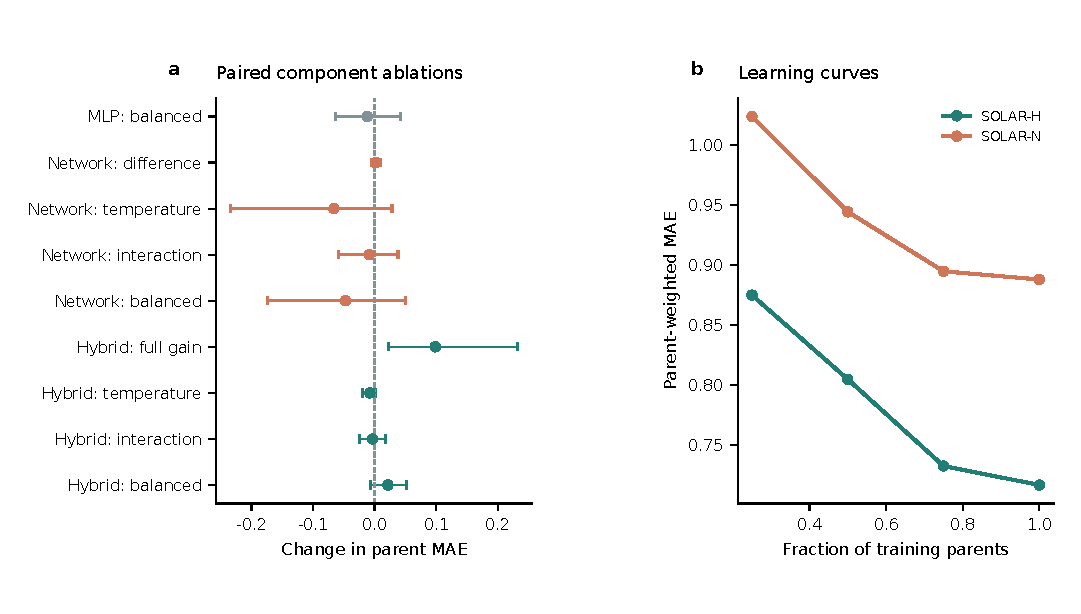
\includegraphics[width=\linewidth]{revision_v2/v2_ablation.pdf}
\caption{组件与数据规模分析。\textbf{a} 组件变体相对完整模型的配对母体误差差及95\% bootstrap区间；Full gain将温度增益恢复为1；MLP的均衡变体以普通MLP为参考。\textbf{b} 按母体抽取25\%、50\%、75\%及100\%训练数据的学习曲线，点为三个种子合并五折评价后的均值。两组实验分别考察组件取舍和独立药物覆盖对预测的影响。}
\label{fig:v2ablation}\end{figure}
\subsection{灵敏度与误差结构}
组件消融进一步引出参数强度的影响。图\ref{fig:v2sensitivity}中，SOLAR-N随差分权重变化的母体等权MAE为[0.8843, 0.8867]，SOLAR-H$_0$随斜率正则化变化的误差为[0.8162, 0.8494]；另行改变SOLAR-N宽度时，误差范围为[0.8455, 0.8964]。差分权重跨多个数量级时误差变化较小，而网络宽度的影响更大，说明当前网络的主要约束更可能来自表示容量与结构覆盖的匹配；固定增益模型即使加强斜率正则化，仍未达到SOLAR-H的母体误差水平，提示直接控制温度分支输出幅度具有额外作用。
\begin{figure}[htbp]\centering
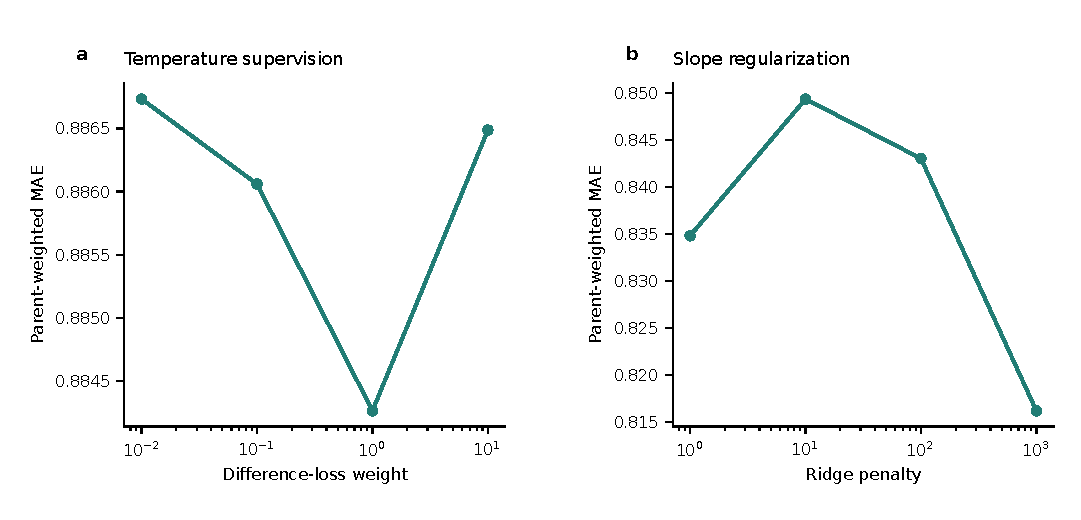
\includegraphics[width=\linewidth]{revision_v2/v2_sensitivity.pdf}
\caption{条件监督与斜率正则化的灵敏度。\textbf{a} 改变SOLAR-N的差分损失权重。\textbf{b} 改变SOLAR-H$_0$的岭回归惩罚。其余参数保持各外层折选定配置，纵轴为三个种子的平均母体等权MAE。差分权重曲线较平缓，斜率正则化曲线呈非单调变化。}
\label{fig:v2sensitivity}\end{figure}
在参数层面的比较之后，图\ref{fig:v2errors}定位了SOLAR-H的误差分布。观测--预测图中，低溶解度端的预测向中心收缩，对应稀疏尾部样本的分辨能力较弱；单条记录跨种子的平均绝对误差最高为3.675。母体误差累积分布则将这种局部大误差与多数药物的表现区分开来。最大训练结构相似度与逐行绝对误差的Spearman系数为-0.062，表明相似结构也可能出现不同幅度的误差；因此，相似度适合作为结构接近程度的描述，不能直接替代预测误差评价。
\begin{figure}[htbp]\centering
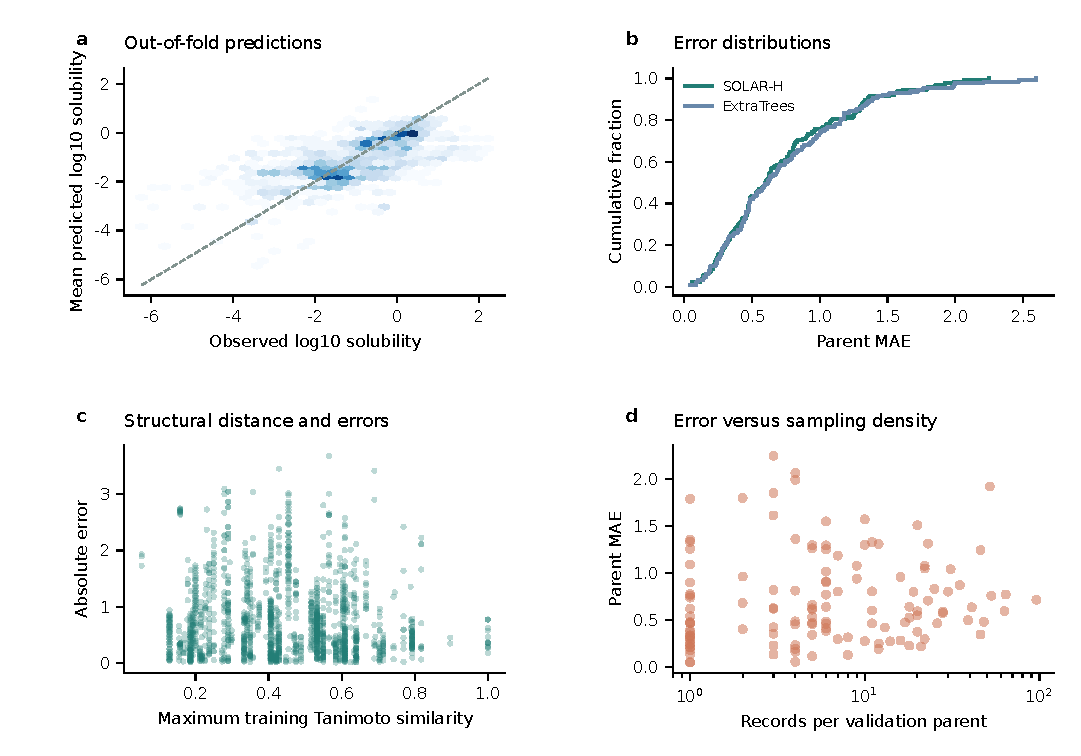
\includegraphics[width=\linewidth]{revision_v2/v2_errors.pdf}
\caption{主要提出方法的折外误差。\textbf{a} 观测与三个种子平均预测的hexbin图，虚线为一致线。\textbf{b} 母体误差的经验累积分布。\textbf{c} 最大训练结构相似度与逐行误差。\textbf{d} 验证母体记录量与母体误差。误差先在各训练种子计算绝对值后平均，区别于平均预测的绝对误差。低溶解度端偏离一致线，结构相似度与误差关系较弱。}
\label{fig:v2errors}\end{figure}
\subsection{结构与温度分支的可解释性}
误差分析描述预测偏差的位置，特征归因进一步考察模型依赖的信息。部署的SOLAR-H选择$\gamma=0$，其温度贡献及温度置换增量均为零。TreeSHAP作用于实际结构树分支，温度头贡献直接由$\gamma\tau r(z)$计算。结构分支平均绝对贡献最大的三个输入为\texttt{drug\_HBA}、\texttt{drug\_TPSA}、\texttt{drug\_RingCount}。SHAP贡献与期望值之和重构结构基线的最大绝对误差为$6.66\times10^{-15}$。

SOLAR-N采用1024段梯形数值积分计算积分梯度，参考输入为标准化描述符零向量和中心温度。完整网络的平均绝对归因最高的输入为\texttt{drug\_HBA}、\texttt{drug\_MolLogP}、\texttt{drug\_TPSA}；归因总和与相对基准预测差的最大误差为0.00522。图\ref{fig:v2explanations}c将单个预测展开为结构基准与各特征贡献，显示局部结果由多项结构信息共同形成；图\ref{fig:v2explanations}d的整组置换进一步显示，打乱药物描述符带来的误差增加大于打乱溶剂或温度。两种归因方法均将氢键受体数与极性相关描述符排在前列，说明模型主要利用分子极性和氢键能力区分溶解度；该解释与SOLAR-H将结构基线作为主要预测分量的设计一致。
\begin{figure}[htbp]\centering
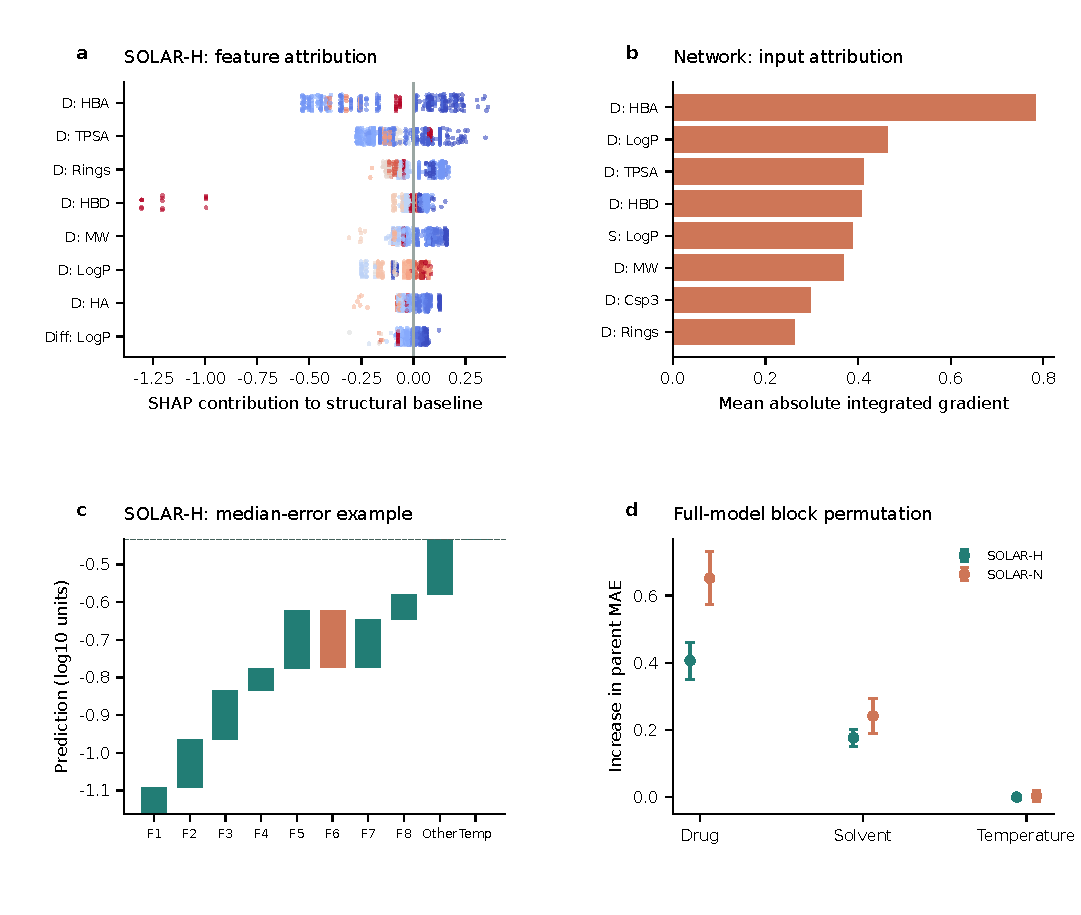
\includegraphics[width=\linewidth]{revision_v2/v2_explanations.pdf}
\caption{提出模型的可解释性。\textbf{a} 混合模型结构基线的前八项平均绝对SHAP特征，红色为高特征值、蓝色为低特征值；D、S、Prod、Diff分别表示药物、溶剂、乘积与绝对差。\textbf{b} SOLAR-N完整预测的积分梯度。\textbf{c} 固定评价集中混合模型绝对误差居中的样本，F1--F8对应a中顺序，Other汇总其余结构特征，Temp为温度头；起点为结构分支期望值。\textbf{d} 完整模型的特征组置换，点与误差线为20次置换的均值和标准差。解释样本为相同397条固定评价记录。全局排序、局部贡献与整组置换从不同尺度描述模型的信息依赖。}
\label{fig:v2explanations}\end{figure}
\subsection{温度关联与因果敏感性}
温度在预测中的贡献较小，还需结合组合内关联解释。图\ref{fig:v2causal}a给出分析假设：药物与溶剂结构影响测量温度的选择和溶解度，未测因素$U$同时影响二者。本文在开发数据上拟合组合固定效应模型$y_{ic}=\alpha_c+\beta T_{ic}+\epsilon_{ic}$，使用组合内去均值估计共同斜率。
157种具有温度变化的组合包含1118条记录、73个母体。在这些相同样本中，未调整组合的斜率为-0.00746，组合内斜率为0.01538；后者的母体bootstrap区间为[0.01236, 0.01902]。逐一移除母体后的斜率范围为[0.01424, 0.01599]，逐一剔除后仍保持正关联。
进一步用偏$R^2$表示潜在未测变量的强度。设$R_T^2$为$U$与温度在控制组合后的偏$R^2$，$R_Y^2$为$U$与结果在控制组合和温度后的偏$R^2$，则遗漏变量导致的点估计偏差大小为\cite{sensitivity2020}
\begin{equation}
|\mathrm{bias}|=\mathrm{SE}_{\mathrm{OLS}}(\hat\beta)
\sqrt{\mathrm{df}\frac{R_Y^2R_T^2}{1-R_T^2}}.
\end{equation}
当两种关联强度相同，偏$R^2$约为0.540即可将当前正斜率调整至零。该数值刻画点估计对假设混杂的敏感性。该分析估计控制组合后的温度关联；实验来源、pH和固态信息未被观测，其潜在混杂作用由图\ref{fig:v2causal}c中的敏感性曲面表征。图\ref{fig:v2causal}揭示总体温度关联与组合内关联方向不同，说明药物和溶剂组成会影响温度趋势的解释；图\ref{fig:v2causal}d中的组合温度序列刻画局部响应，而SOLAR-H的增益由未见母体上的验证误差决定。两者分别对应组合内拟合与跨药物迁移，因而正温度关联与较小预测增益可以同时出现。
\begin{figure}[htbp]\centering
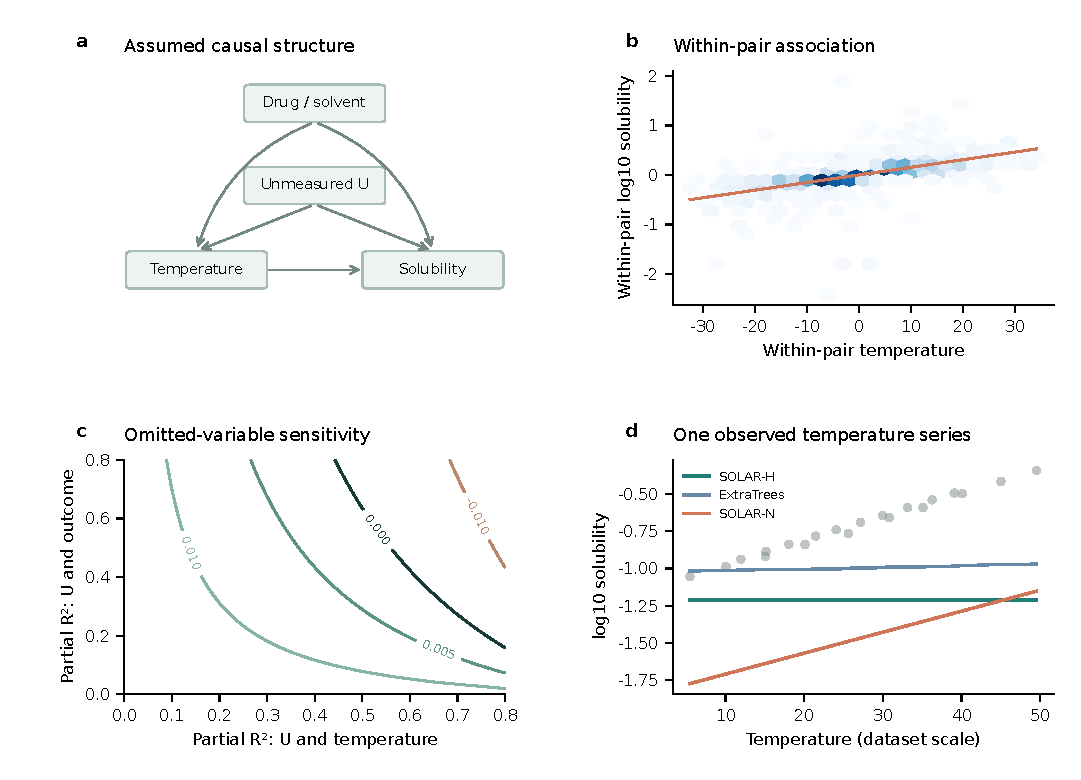
\includegraphics[width=\linewidth]{revision_v2/v2_causal.pdf}
\caption{温度关联、混杂敏感性与模型响应。\textbf{a} 分析采用的假设DAG。\textbf{b} 开发数据组合内去均值后的分布及共同斜率。\textbf{c} 未测变量不同偏$R^2$强度下向零方向调整的系数等高线，零线对应消除正关联所需的组合强度。\textbf{d} 温度覆盖较充分的一种开发组合的观测与模型响应。组合内斜率、混杂敏感性与单组合响应分别呈现温度分析的统计、假设和局部层面。}
\label{fig:v2causal}\end{figure}
